\documentclass{notes}
\usetikzlibrary{shapes, shapes.geometric}
\usepackage{multirow,bigdelim}

\class{CS 181 (Introduction to Formal Languages and Automata Theory)}

\begin{document}

\section{Deterministic finite automata (DFAs)}

\subsection{Basic notions}

\begin{defn}
  An \textbf{alphabet} is any finite set of symbols.
\end{defn}

\begin{eg}
  Binary alphabet: $\left \{ \verb~0~, \verb~1~ \right \}$
\end{eg}

\begin{eg}
  English alphabet: $\left \{ \verb~a~, \verb~b~, \dots, \verb~c~ \right \}$
\end{eg}

\begin{defn}
  A \textbf{string} is any finite sequence of symbols from a given alphabet.
\end{defn}

\begin{eg}
  \verb~001010110101~
\end{eg}

\begin{eg}
  \verb~abracadabra~
\end{eg}

\begin{eg}
  $\varepsilon$ (empty string)
\end{eg}

\begin{defn}
  A \textbf{language} is a set of strings over a given alphabet.
\end{defn}

\begin{eg}
  $\varnothing$ (empty language)
\end{eg}

\begin{eg}
  $\left \{ \varepsilon \right \}$
\end{eg}

\begin{eg}
  $\left \{ \verb~acclaim~, \verb~aim~, \verb~brim~, \dots \right \}$
\end{eg}

\begin{eg}
  $\left \{ \verb~0~, \verb~1~, \verb~00~, \verb~11~, \dots \right \}$
\end{eg}

\begin{defn}
  A \textbf{computational device} is a mechanism that inputs a string and either accepts or rejects it.
\end{defn}

\subsection{Deterministic finite automata}

\begin{itemize}
  \item Choose an alphabet: $\left \{ \verb~a~, \verb~b~ \right \}$.
  \item Draw states.
  \item Choose start state and accept states.
  \item Draw transitions (out of every state on every symbol).
\end{itemize}

\begin{minipage}{0.5 \textwidth}
  \begin{center}
    \begin{tikzpicture}[> = stealth, node distance = 3em]
      \node[initial, initial text=, state, minimum size = 2em] (q1) {};
      \node[below left = of q1, accepting, state, minimum size = 2em] (q2) {};
      \node[below right = of q1, accepting, state, minimum size = 2em] (q3) {};
      \node[below right = of q2, state, minimum size = 2em] (q4) {};
      \draw[->]
      (q1) edge[above left] node{\verb~a~} (q2)
      (q1) edge[above right] node{\verb~b~} (q3)
      (q2) edge[loop left] node{\verb~a~} (q2)
      (q2) edge[below left] node{\verb~b~} (q4)
      (q3) edge[below right] node{\verb~a~} (q4)
      (q3) edge[loop right] node{\verb~b~} (q3)
      (q4) edge[loop below] node{\verb~a~,\verb~b~} (q4)
      ;
    \end{tikzpicture}
  \end{center}
\end{minipage}%
\begin{minipage}{0.5 \textwidth}
  \begin{center}
    \begin{tabular}{cc}
      Input & Output \\ 
      \hline
      $\varepsilon$ & reject \\ 
      \verb~ab~ & reject \\ 
      \verb~aaa~ & accept \\ 
      \verb~bb~ & accept
    \end{tabular}
  \end{center}
\end{minipage}

In words, this machine accepts nonempty strings of all \verb~a~'s or all \verb~b~'s.

\begin{defn}
  The \textbf{language} of a DFA is the set of all strings it accepts.
\end{defn}

\begin{eg}
  
  \begin{minipage}{0.5 \textwidth}
    \begin{center}
      \begin{tikzpicture}[> = stealth, node distance = 3em]
        \node[accepting, initial, initial text=, state, minimum size = 2em] (q1) at (90 : 1.5) {};
        \node[state, minimum size = 2em] (q2) at (330 : 1.5) {};
        \node[state, minimum size = 2em] (q3) at (210 : 1.5) {};
        \draw[->]
        (q1) edge[loop above] node{\verb~0~} (q1)
        (q1) edge[below left] node{\verb~1~} (q2)
        (q1) edge[bend right, above left] node{\verb~2~} (q3)
        (q2) edge[loop right] node{\verb~0~} (q2)
        (q2) edge[above] node{\verb~1~} (q3)
        (q2) edge[bend right, above right] node{\verb~2~} (q1)
        (q3) edge[loop left] node{\verb~0~} (q3)
        (q3) edge[below right] node{\verb~1~} (q1)
        (q3) edge[bend right, below] node{\verb~2~} (q2)
        ;
      \end{tikzpicture}
    \end{center}
  \end{minipage}%
  \begin{minipage}{0.5 \textwidth}
    \begin{center}
      \begin{tabular}{cc}
        Input & Output \\ 
        \hline
        \verb~00...0~ & accept \\ 
        \verb~12~ & accept \\ 
        \verb~111~ & accept \\ 
        \verb~20~ & reject \\ 
        \verb~1~ & reject
      \end{tabular}
    \end{center}
  \end{minipage}

  \begin{center}
    $\Sigma = \left \{ \verb~0~, \verb~1~, \verb~2~ \right \}$, $\mathcal L = \left \{ w : 3 \mid \sum w_i \right \}$
  \end{center}
\end{eg}

\begin{eg}
  \begin{center}
    \begin{tikzpicture}[> = stealth, node distance = 3em]
      \node[accepting, initial, initial text=, state, minimum size = 2em] (q1) {};
      \node[right = of q1, state, minimum size = 2em] (q2) {};
      \draw[->]
      (q1) edge[bend right, below] node{\verb~0~,\verb~1~} (q2)
      (q2) edge[bend right, above] node{\verb~0~,\verb~1~} (q1)
      ;
    \end{tikzpicture}

    $\Sigma = \left \{ \verb~0~, \verb~1~ \right \}$, $\mathcal L = \left \{ w : 2 \mid \left | w \right | \right \}$
  \end{center}
\end{eg}

\begin{eg}
  \begin{center}
    \begin{tikzpicture}[> = stealth, node distance = 3em]
      \node[initial, initial text=, state, minimum size = 2em] (q1) {};
      \node[accepting, below left = of q1, state, minimum size = 2em] (q2) {};
      \node[below = of q2, state, minimum size = 2em] (q3) {};
      \node[accepting, below right = of q1, state, minimum size = 2em] (q4) {};
      \node[below = of q4, state, minimum size = 2em] (q5) {};
      \draw[->]
      (q1) edge[above left] node{\verb~a~} (q2)
      (q1) edge[above right] node{\verb~b~} (q4)
      (q2) edge[loop left] node{\verb~a~} (q2)
      (q2) edge[bend right, left] node{\verb~b~} (q3)
      (q3) edge[bend right, right] node{\verb~a~} (q2)
      (q3) edge[loop below] node{\verb~b~} (q3)
      (q4) edge[bend right, left] node{\verb~a~} (q5)
      (q4) edge[loop right] node{\verb~b~} (q4)
      (q5) edge[loop below] node{\verb~a~} (q5)
      (q5) edge[bend right, right] node{\verb~b~} (q4)
      ;
    \end{tikzpicture}

    $\Sigma = \left \{ \verb~a~, \verb~b~ \right \}$, $\mathcal L = \left \{ w : w \neq \varepsilon \land w_1 = w_{\left | w \right |  } \right \}$
  \end{center}
\end{eg}

\subsection{Designing DFAs}

We will be using the binary alphabet $\left \{ \verb~0~, \verb~1~ \right \}$.

\begin{eg}
  Design a DFA for $\mathcal L = \varnothing$.
  
  \begin{center}
    \begin{tikzpicture}[> = stealth, node distance = 3em]
      \node[initial, initial text=, state, minimum size = 2em] (q1) {};
      \draw[->]
      (q1) edge[loop right] node{\verb~0~,\verb~1~} (q1)
      ;
    \end{tikzpicture}
  \end{center}
\end{eg}

\begin{eg}
  Design a DFA for $\mathcal L = \left \{ w : \text{every odd position is a \verb~1~} \right \}$.
  
  \begin{center}
    \begin{tikzpicture}[> = stealth, node distance = 3em]
      \node[accepting, initial, initial text=, state, minimum size = 2em] (q1) {};
      \node[accepting, below right = of q1, state, minimum size = 2em] (q2) {};
      \node[above right = of q1, state, minimum size = 2em] (q3) {};
      \draw[->]
      (q1) edge[above left] node{\verb~0~} (q3)
      (q1) edge[bend right, below left] node{\verb~1~} (q2)
      (q2) edge[bend right, above right] node{\verb~0~,\verb~1~} (q1)
      (q3) edge[loop right] node{\verb~0~,\verb~1~} (q3)
      ;
    \end{tikzpicture}
  \end{center}
\end{eg}

\begin{eg}
  Design a DFA for $\mathcal L = \left \{ w : \text{$w$ ends in \verb~0~} \right \}$.
  
  \begin{center}
    \begin{tikzpicture}[> = stealth, node distance = 3em]
      \node[initial, initial text=, state, minimum size = 2em] (q1) {};
      \node[right = of q1, accepting, state, minimum size = 2em] (q2) {};
      \draw[->]
      (q1) edge[bend right, below] node{\verb~0~} (q2)
      (q1) edge[loop above] node{\verb~1~} (q1)
      (q2) edge[loop below] node{\verb~0~} (q2)
      (q2) edge[bend right, above] node{\verb~1~} (q1)
      ;
    \end{tikzpicture}
  \end{center}
\end{eg}

\begin{eg}
  Design a DFA for $\mathcal L = \left \{ w : \text{$w$ begins with \verb~1~, ends with \verb~0~} \right \}$.
  
  \begin{center}
    \begin{tikzpicture}[> = stealth, node distance = 3em]
      \node[initial, initial text=, state, minimum size = 2em] (q1) {};
      \node[above right = of q1, state, minimum size = 2em] (q2) {};
      \node[right = of q2, accepting, state, minimum size = 2em] (q3) {};
      \node[below right = of q1, state, minimum size = 2em] (q4) {};
      \draw[->]
      (q1) edge[below left] node{\verb~0~} (q4)
      (q1) edge[above left] node{\verb~1~} (q2)
      (q2) edge[bend right, below] node{\verb~0~} (q3)
      (q2) edge[loop above] node{\verb~1~} (q2)
      (q3) edge[loop right] node{\verb~0~} (q3)
      (q3) edge[bend right, above] node{\verb~1~} (q2)
      (q4) edge[loop right] node{\verb~0~,\verb~1~} (q4)
      ;
    \end{tikzpicture}
  \end{center}
\end{eg}

\begin{eg}
  Design a DFA for $\mathcal L = \left \{ w : \left | w \right | \leq 4  \right \}$.
  
  \begin{center}
    \begin{tikzpicture}[> = stealth, node distance = 3em]
      \node[accepting, initial, initial text=, state, minimum size = 2em] (q1) {};
      \node[right = of q1, accepting, state, minimum size = 2em] (q2) {};
      \node[accepting, right = of q2, state, minimum size = 2em] (q3) {};
      \node[accepting, right = of q3, state, minimum size = 2em] (q4) {};
      \node[accepting, right = of q4, state, minimum size = 2em] (q5) {};
      \node[right = of q5, state, minimum size = 2em] (q6) {};
      \draw[->]
      (q1) edge[above] node{\verb~0~,\verb~1~} (q2)
      (q2) edge[above] node{\verb~0~,\verb~1~} (q3)
      (q3) edge[above] node{\verb~0~,\verb~1~} (q4)
      (q4) edge[above] node{\verb~0~,\verb~1~} (q5)
      (q5) edge[above] node{\verb~0~,\verb~1~} (q6)
      (q6) edge[loop right] node{\verb~0~,\verb~1~} (q6)
      ;
    \end{tikzpicture}
  \end{center}
\end{eg}

\newpage

\begin{eg}
  Design a DFA for $\mathcal L = \left \{ w : 1000 \mid \left | w \right | \right \}$.
  
  In words, each state represents a remainder modulo 1000, and only the 0 state is accepting.
\end{eg}

\begin{eg}
  Design a DFA for $\mathcal L = \left \{ w : \text{$w$ contains \verb~0101~ as a substring} \right \}$.
  
  \begin{center}
    \begin{tikzpicture}[> = stealth, node distance = 3em]
      \node[initial, initial text=, state, minimum size = 2em] (q1) {$\varepsilon$};
      \node[right = of q1, state, minimum size = 2em] (q2) {\verb~0~};
      \node[right = of q2, state, minimum size = 2em] (q3) {\verb~01~};
      \node[right = of q3, state, minimum size = 2em] (q4) {\verb~010~};
      \node[accepting, right = of q4, state, minimum size = 2em] (q5) {\verb~0101~};
      \draw[->]
      (q1) edge[above] node{\verb~0~} (q2)
      (q1) edge[loop above] node{\verb~1~} (q1)
      (q2) edge[loop above] node{\verb~0~} (q2)
      (q2) edge[above] node{\verb~1~} (q3)
      (q3) edge[above] node{\verb~0~} (q4)
      (q3) edge[bend right = 75, above] node{\verb~1~} (q1)
      (q4) edge[bend right = 60, above] node{\verb~0~} (q2)
      (q4) edge[above] node{\verb~1~} (q5)
      (q5) edge[loop right] node{\verb~0~,\verb~1~} (q5)
      ;
    \end{tikzpicture}
  \end{center}
\end{eg}

\begin{eg}[Week 1 Discussion]
  Design a DFA for $\mathcal L = \left \{ w : \left | w \right | > 0 \land \text{$w$ contains only \verb~1~s} \right \}$.
  
  \begin{center}
    \begin{tikzpicture}[> = stealth, node distance = 3em]
      \node[initial, initial text=, state, minimum size = 2em] (q1) {};
      \node[right = of q1, accepting, state, minimum size = 2em] (q2) {};
      \node[right = of q2, state, minimum size = 2em] (q3) {};
      \draw[->]
      (q1) edge[bend right, below] node{\verb~0~} (q3)
      (q1) edge[above] node{\verb~1~} (q2)
      (q2) edge[above] node{\verb~0~} (q3)
      (q2) edge[loop above] node{\verb~1~} (q2)
      (q3) edge[loop right] node{\verb~0~,\verb~1~} (q3)
      ;
    \end{tikzpicture}
  \end{center}
\end{eg}

\begin{eg}[Week 1 Discussion]
  Design a DFA for $\mathcal L = \left \{ w : \text{$w$ ends in \verb~1101~} \right \}$.
  
  \begin{center}
    \begin{tikzpicture}[> = stealth, node distance = 3em]
      \node[initial, initial text=, state, minimum size = 2em] (q1) {};
      \node[right = of q1, state, minimum size = 2em] (q2) {};
      \node[right = of q2, state, minimum size = 2em] (q3) {};
      \node[right = of q3, state, minimum size = 2em] (q4) {};
      \node[accepting, right = of q4, state, minimum size = 2em] (q5) {};
      \draw[->]
      (q1) edge[loop below] node{\verb~0~} (q1)
      (q1) edge[bend right, below] node{\verb~1~} (q2)
      (q2) edge[bend right, above] node{\verb~0~} (q1)
      (q2) edge[above] node{\verb~1~} (q3)
      (q3) edge[above] node{\verb~0~} (q4)
      (q3) edge[loop above] node{\verb~1~} (q3)
      (q4) edge[bend right = 60, above] node{\verb~0~} (q1)
      (q4) edge[above] node{\verb~1~} (q5)
      (q5) edge[bend right = 75, above] node{\verb~0~} (q1)
      (q5) edge[bend right, above] node{\verb~1~} (q3)
      ;
    \end{tikzpicture}
  \end{center}
\end{eg}

\begin{eg}[Week 1 Discussion]
  Design a DFA for $\mathcal L = \left \{ w : \text{$w$ contains \verb~1101~} \right \}$.
  
  \begin{center}
    \begin{tikzpicture}[> = stealth, node distance = 3em]
      \node[initial, initial text=, state, minimum size = 2em] (q1) {};
      \node[right = of q1, state, minimum size = 2em] (q2) {};
      \node[right = of q2, state, minimum size = 2em] (q3) {};
      \node[right = of q3, state, minimum size = 2em] (q4) {};
      \node[accepting, right = of q4, state, minimum size = 2em] (q5) {};
      \draw[->]
      (q1) edge[loop below] node{\verb~0~} (q1)
      (q1) edge[bend right, below] node{\verb~1~} (q2)
      (q2) edge[bend right, above] node{\verb~0~} (q1)
      (q2) edge[above] node{\verb~1~} (q3)
      (q3) edge[above] node{\verb~0~} (q4)
      (q3) edge[loop above] node{\verb~1~} (q3)
      (q4) edge[bend right = 60, above] node{\verb~0~} (q1)
      (q4) edge[above] node{\verb~1~} (q5)
      (q5) edge[loop right] node{\verb~0~,\verb~1~} (q5)
      ;
    \end{tikzpicture}
  \end{center}
\end{eg}

\newpage

\subsection{Formal definitions}

\begin{defn}
  A DFA is a tuple $(Q, \Sigma, \delta, q_{0}, F)$
  where
  \begin{itemize}
    \item $Q =$ set of states, 
    \item $\Sigma =$ alphabet, 
    \item $\delta =$ transition function ($\delta \colon Q \times \Sigma \to Q$), 
    \item $q_0 =$ start state ($q_0 \in Q$), and 
    \item $F =$ set of accept states ("favorable"? states, $F \subseteq Q$).
  \end{itemize}
\end{defn}

\begin{eg}
  A formal description of the DFA

  \begin{center}
    \begin{tikzpicture}[> = stealth, node distance = 3em]
      \node[initial, initial text=, state, minimum size = 2em] (q1) {$A$};
      \node[accepting, right = of q1, accepting, state, minimum size = 2em] (q2) {$B$};
      \node[right = of q2, state, minimum size = 2em] (q3) {$C$};
      \draw[->]
      (q1) edge[loop above] node{\verb~0~} (q1)
      (q1) edge[above] node{\verb~1~} (q2)
      (q2) edge[bend right, below] node{\verb~0~} (q3)
      (q2) edge[loop above] node{\verb~1~} (q2)
      (q3) edge[bend right, above] node{\verb~0~,\verb~1~} (q2)
      ;
    \end{tikzpicture}
  \end{center}
  
  is given by $(\left \{ A, B, C \right \}, \left \{ \verb~0~, \verb~1~ \right \}, \delta, A, \left \{ B \right \})$ where $\delta$ is defined by the table
  \begin{center}
    \begin{tabular}{c|cc}
      & \verb~0~ & \verb~1~ \\ 
      \hline
      $A$ & $A$ & $B$ \\ 
      $B$ & $C$ & $B$ \\ 
      $C$ & $B$ & $B$.
    \end{tabular}
  \end{center}
\end{eg}

\begin{eg}
  The graph for the DFA $(\left \{ A, B, C, D, E \right \}, \left \{ \verb~0~, \verb~1~ \right \}, \delta, C, \left \{ C \right \})$ where $\delta$ is defined by the table 
  \begin{center}
    \begin{tabular}{c|cc}
      & \verb~0~ & \verb~1~ \\ 
      \hline
      $A$ & $A$ & $B$ \\ 
      $B$ & $A$ & $C$ \\ 
      $C$ & $B$ & $D$ \\ 
      $D$ & $C$ & $E$ \\ 
      $E$ & $D$ & $E$
    \end{tabular}
  \end{center}
  
  is given by: 
  
  \begin{center}
    \begin{tikzpicture}[> = stealth, node distance = 3em]
      \node[state, minimum size = 2em] (q1) {$A$};
      \node[right = of q1, state, minimum size = 2em] (q2) {$B$};
      \node[accepting, initial above, initial text=, right = of q2, state, minimum size = 2em] (q3) {$C$};
      \node[right = of q3, state, minimum size = 2em] (q4) {$D$};
      \node[right = of q4, state, minimum size = 2em] (q5) {$E$};
      \draw[->]
      (q1) edge[loop left] node{\verb~0~} (q1)
      (q1) edge[bend right, below] node{\verb~1~} (q2)
      (q2) edge[bend right, above] node{\verb~0~} (q1)
      (q2) edge[bend right, below] node{\verb~1~} (q3)
      (q3) edge[bend right, above] node{\verb~0~} (q2)
      (q3) edge[bend right, below] node{\verb~1~} (q4)
      (q4) edge[bend right, above] node{\verb~0~} (q3)
      (q4) edge[bend right, below] node{\verb~1~} (q5)
      (q5) edge[bend right, above] node{\verb~0~} (q4)
      (q5) edge[loop right] node{\verb~1~} (q5)
      ;
    \end{tikzpicture}
  \end{center}
\end{eg}

\begin{eg}
  A formal description for Example~\ref{eg:1.3.6} is given by $(\left \{ 0, 1, 2, \dots, 999 \right \}, \left \{ \verb~0~, \verb~1~ \right \}, \delta, 0, \left \{ 0 \right \})$ where $\delta(q, \sigma) = (q + 1) \mod 1000$.
\end{eg}

\newpage

\begin{defn}
  DFA $(Q, \Sigma, \delta, q_{0}, F)$ {\boldmath \bfseries accepts} a string $w = w_1 w_2 \dots w_n$ iff
  \[
    \delta(\cdots \delta(\delta(q_0, w_1), w_2) \cdots, w_n) \in F.
  \]
\end{defn}

\begin{defn}
  DFA $D$ {\boldmath \bfseries recognizes} the language $\mathcal L$ iff 
  \[
    \mathcal L = \left \{ w : \text{$D$ accepts $w$} \right \}.
  \]
\end{defn}

\begin{note}
  \begin{itemize}
    \item Every DFA recognizes exactly 1 language.

    \item A language has either 0 or $\infty$ DFAs recognizing it.
  \end{itemize}
\end{note}

\section{Nondeterminism}

\subsection{Basic notions}

\begin{eg}
  \begin{center}
    \begin{tikzpicture}[> = stealth, node distance = 3em]
      \node[initial, initial text=, state, minimum size = 2em] (q1) {$A$};
      \node[right = of q1, state, minimum size = 2em] (q2) {$B$};
      \node[right = of q2, state, minimum size = 2em] (q3) {$C$};
      \node[accepting, right = of q3, state, minimum size = 2em] (q4) {$D$};
      \draw[->]
      (q1) edge[loop above] node{\verb~0~,\verb~1~} (q1)
      (q1) edge[above] node{\verb~1~} (q2)
      (q2) edge[above] node{\verb~0~,$\varepsilon$} (q3)
      (q3) edge[above] node{\verb~1~} (q4)
      (q4) edge[loop above] node{\verb~0~,\verb~1~} (q4)
      ;
    \end{tikzpicture}
  \end{center}

  \begin{itemize}
    \item Choose an alphabet: $\left \{ \verb~0~, \verb~1~ \right \}$.

    \item Draw states.
      
    \item Choose start state and accept states.
    The steps so far are the same as those of a DFA.
      
    \item Draw transitions.
    A state may have any number of transitions on a given symbol.
    A state may also have transitions on $\varepsilon$.
  \end{itemize}
\end{eg}

\begin{defn}
  An NFA {\boldmath \bfseries accepts} $w$ iff there is \textit{at least} one path to an accept state.
\end{defn}

\newpage

\begin{eg}
  The output table for Example~\ref{eg:2.1.1} is given by 
  \begin{center}
    \begin{tabular}{ccc}
      Input & Accepting path & Output \\ 
      \hline
      $\varepsilon$ & - & reject \\ 
      \verb~0~ & - & reject \\ 
      \verb~1~ & - & reject \\ 
      \verb~010110~ & $AABCDDD$ & accept \\
      \verb~010~ & - & reject \\ 
      \verb~11~ & $ABCD$ & accept. 
    \end{tabular}
  \end{center}
  
  Then the language is the set of all strings containing \verb~101~ or \verb~11~.
\end{eg}

\subsection{Using shortcuts}

\begin{eg}
  Design an NFA for $\mathcal L = \varnothing$.
  
  \begin{center}
    \begin{tikzpicture}[> = stealth, node distance = 3em]
      \node[initial, initial text=, state, minimum size = 2em] (q1) {};
      \draw[->]
      ;
    \end{tikzpicture}
  \end{center}
\end{eg}

\begin{eg}
  Design an NFA for $\mathcal L = \left \{ \varepsilon \right \}$.

  \begin{center}
    \begin{tikzpicture}[> = stealth, node distance = 3em]
      \node[accepting, initial, initial text=, state, minimum size = 2em] (q1) {};
      \draw[->]
      ;
    \end{tikzpicture}
  \end{center}
\end{eg}

\begin{eg}
  Design an NFA for $\mathcal L = \left \{ w : \text{$w$ doesn't contain \verb~1~} \right \}$.

  \begin{center}
    \begin{tikzpicture}[> = stealth, node distance = 3em]
      \node[accepting, initial, initial text=, state, minimum size = 2em] (q1) {};
      \draw[->]
      (q1) edge[loop right] node{\verb~0~} (q1)
      ;
    \end{tikzpicture}
  \end{center}
\end{eg}

\begin{eg}
  Design an NFA for $\mathcal L = \left \{ w : \text{$\left | w \right | \geq 2$ and $w$ starts and ends with \verb~0~} \right \}$.
  
  \begin{center}
    \begin{tikzpicture}[> = stealth, node distance = 3em]
      \node[initial, initial text=, state, minimum size = 2em] (q1) {};
      \node[right = of q1, state, minimum size = 2em] (q2) {};
      \node[accepting, right = of q2, state, minimum size = 2em] (q3) {};
      \draw[->]
      (q1) edge[above] node{\verb~0~} (q2)
      (q2) edge[above] node{\verb~0~} (q3)
      (q2) edge[loop above] node{\verb~0~,\verb~1~} (q2)
      ;
    \end{tikzpicture}
  \end{center}
\end{eg}

\subsection{Pattern matching}

\begin{eg}
  Design an NFA for $\mathcal L = \left \{ w : \text{conatins \verb~0101~} \right \}$.
  
  \begin{center}
    \begin{tikzpicture}[> = stealth, node distance = 3em]
      \node[initial, initial text=, state, minimum size = 2em] (q1) {};
      \node[right = of q1, state, minimum size = 2em] (q2) {};
      \node[right = of q2, state, minimum size = 2em] (q3) {};
      \node[right = of q3, state, minimum size = 2em] (q4) {};
      \node[accepting, right = of q4, state, minimum size = 2em] (q5) {};
      \draw[->]
      (q1) edge[loop above] node{\verb~0~,\verb~1~} (q1)
      (q1) edge[above] node{\verb~0~} (q2)
      (q2) edge[above] node{\verb~1~} (q3)
      (q3) edge[above] node{\verb~0~} (q4)
      (q4) edge[above] node{\verb~1~} (q5)
      (q5) edge[loop above] node{\verb~0~,\verb~1~} (q5)
      ;
    \end{tikzpicture}
  \end{center}
\end{eg}

\newpage

\begin{eg}
  Design an NFA for $\mathcal L = \{ w : w = \underbrace{\verb~00...0~}_{\geq 0}\underbrace{\verb~11...1~}_{\geq 0}\underbrace{\verb~00...0~}_{\geq 1} \}$.
  
  \begin{center}
    \begin{tikzpicture}[> = stealth, node distance = 3em]
      \node[initial, initial text=, state, minimum size = 2em] (q1) {};
      \node[right = of q1, state, minimum size = 2em] (q2) {};
      \node[accepting, right = of q2, state, minimum size = 2em] (q3) {};
      \draw[->]
      (q1) edge[loop above] node{\verb~0~} (q1)
      (q1) edge[above] node{$\varepsilon$} (q2)
      (q2) edge[loop above] node{\verb~1~} (q2)
      (q2) edge[above] node{\verb~0~} (q3)
      (q3) edge[loop above] node{\verb~0~} (q3)
      ;
    \end{tikzpicture}
  \end{center}
\end{eg}

\begin{eg}
  Design an NFA for $\mathcal L = \left \{ w : \text{$w$ has a \verb~1~ in the 3rd position from the end} \right \}$.
  
  \begin{center}
    \begin{tikzpicture}[> = stealth, node distance = 3em]
      \node[initial, initial text=, state, minimum size = 2em] (q1) {};
      \node[right = of q1, state, minimum size = 2em] (q2) {};
      \node[right = of q2, state, minimum size = 2em] (q3) {};
      \node[accepting, right = of q3, state, minimum size = 2em] (q4) {};
      \draw[->]
      (q1) edge[loop above] node{\verb~0~,\verb~1~} (q1)
      (q1) edge[above] node{\verb~1~} (q2)
      (q2) edge[above] node{\verb~0~,\verb~1~} (q3)
      (q3) edge[above] node{\verb~0~,\verb~1~} (q4)
      ;
    \end{tikzpicture}
  \end{center}
\end{eg}

\begin{eg}[Week 1 Discussion]
  Design an NFA for $\mathcal L = \left \{ w : \text{$w$ contains \verb~1101~} \right \}$.
  
  \begin{center}
    \begin{tikzpicture}[> = stealth, node distance = 3em]
      \node[initial, initial text=, state, minimum size = 2em] (q1) {};
      \node[right = of q1, state, minimum size = 2em] (q2) {};
      \node[right = of q2, state, minimum size = 2em] (q3) {};
      \node[right = of q3, state, minimum size = 2em] (q4) {};
      \node[accepting, right = of q4, state, minimum size = 2em] (q5) {};
      \draw[->]
      (q1) edge[loop above] node{\verb~0~,\verb~1~} (q1)
      (q1) edge[above] node{\verb~1~} (q2)
      (q2) edge[above] node{\verb~1~} (q3)
      (q3) edge[above] node{\verb~0~} (q4)
      (q4) edge[above] node{\verb~1~} (q5)
      (q5) edge[loop above] node{\verb~0~,\verb~1~} (q5)
      ;
    \end{tikzpicture}
  \end{center}
\end{eg}

\begin{eg}[Week 1 Discussion]
  Design an NFA for $\mathcal L = \{ w : w = \underbrace{\verb~11...1~}_{\geq 0}\underbrace{\verb~00...0~}_{\geq 1}\underbrace{\verb~11...1~}_{\geq 0} \}$.
  
  \begin{center}
    \begin{tikzpicture}[> = stealth, node distance = 3em]
      \node[initial, initial text=, state, minimum size = 2em] (q1) {};
      \node[right = of q1, state, minimum size = 2em] (q2) {};
      \node[accepting, right = of q2, state, minimum size = 2em] (q3) {};
      \draw[->]
      (q1) edge[loop above] node{\verb~1~} (q1)
      (q1) edge[above] node{$\varepsilon$} (q2)
      (q2) edge[loop above] node{\verb~0~} (q2)
      (q2) edge[above] node{\verb~0~} (q3)
      (q3) edge[loop above] node{\verb~1~} (q3)
      ;
    \end{tikzpicture} 
  \end{center}
\end{eg}

\subsection{Alternatives}

\begin{eg}
  Design an NFA for $\mathcal L = \left \{ w : 2 \mid \left | w \right | \lor 3 \mid \left | w \right | \right \}$.
  
  \begin{center}
    \begin{tikzpicture}[> = stealth, node distance = 3em]
      \node[initial, initial text=, state, minimum size = 2em] (q1) {};
      \node[accepting, above right = of q1, state, minimum size = 2em] (q2) {};
      \node[right = of q2, state, minimum size = 2em] (q3) {};
      \node[accepting, below right = of q1, state, minimum size = 2em] (q4) {};
      \node[above right = of q4, state, minimum size = 2em] (q5) {};
      \node[below right = of q4, state, minimum size = 2em] (q6) {};
      \draw[->]
      (q1) edge[above left] node{$\varepsilon$} (q2)
      (q2) edge[bend right, below] node{\verb~0~,\verb~1~} (q3)
      (q3) edge[bend right, above] node{\verb~0~,\verb~1~} (q2)
      (q1) edge[below left] node{$\varepsilon$} (q4)
      (q4) edge[above left] node{\verb~0~,\verb~1~} (q5)
      (q5) edge[right] node{\verb~0~,\verb~1~} (q6)
      (q6) edge[below left] node{\verb~0~,\verb~1~} (q4)
      ;
    \end{tikzpicture}
  \end{center}
  
  \newpage
  
  Note that the following is not valid due to side effects: 

  \begin{center}
    \begin{tikzpicture}[> = stealth, node distance = 3em]
      \node[accepting, initial, initial text=, state, minimum size = 2em] (q1) {};
      \node[right = of q1, state, minimum size = 2em] (q2) {};
      \node[accepting, below = of q1, state, minimum size = 2em] (q3) {};
      \node[below left = of q3, state, minimum size = 2em] (q4) {};
      \node[below right = of q3, state, minimum size = 2em] (q5) {};
      \draw[->]
      (q1) edge[bend right, below] node{\verb~0~,\verb~1~} (q2)
      (q2) edge[bend right, above] node{\verb~0~,\verb~1~} (q1)
      (q1) edge[left] node{$\varepsilon$} (q3)
      (q3) edge[above left] node{\verb~0~,\verb~1~} (q4)
      (q4) edge[below] node{\verb~0~,\verb~1~} (q5)
      (q5) edge[above right] node{\verb~0~,\verb~1~} (q3)
      ;
    \end{tikzpicture}
  \end{center}
\end{eg}

\begin{eg}[Week 1 Discussion]
  Design an NFA for \\ $\mathcal L = \{ w : \text{$w$ contains \verb~1101~} \lor w = \underbrace{\verb~11...1~}_{\geq 0}\underbrace{\verb~00...0~}_{\geq 1}\underbrace{\verb~11...1~}_{\geq 0} \}$.
  
  \begin{center}
    \begin{tikzpicture}[> = stealth, node distance = 3em]
      \node[initial, initial text=, state, minimum size = 2em] (q1) {};
      \node[above right = of q1, style = {draw, rectangle, minimum width = 4em, minimum height = 2em}, minimum size = 2em] (q2) {NFA from Example~\ref{eg:2.3.4}};
      \node[below right = of q1, style = {draw, rectangle, minimum width = 4em, minimum height = 2em}, minimum size = 2em] (q3) {NFA from Example~\ref{eg:2.3.5}};
      \draw[->]
      (q1) edge[above left] node{$\varepsilon$} (q2.west)
      (q1) edge[below left] node{$\varepsilon$} (q3.west)
      ;
    \end{tikzpicture}
  \end{center}
\end{eg}

\begin{eg}
  Design an NFA for $\mathcal L = \left \{ w : \text{$w$ contains an even number of \verb~0~s, or exactly two \verb~1~s} \right \}$.
  
  \begin{center}
    \begin{tikzpicture}[> = stealth, node distance = 3em]
      \node[initial, initial text=, state, minimum size = 2em] (1) {};
      \node[above right = of 1, accepting, state, minimum size = 2em] (2) {};
      \node[right = of 2, state, minimum size = 2em] (3) {};
      \node[below right = of 1,state, minimum size = 2em] (4) {};
      \node[right = of 4, state, minimum size = 2em] (5) {};
      \node[accepting, right = of 5, state, minimum size = 2em] (6) {};
      \draw[->]
      (1) edge[above left] node{$\varepsilon$} (2)
      (1) edge[below left] node{$\varepsilon$} (4)
      (2) edge[bend right, below] node{\verb~0~} (3)
      (2) edge[loop above] node{\verb~1~} (2)
      (3) edge[bend right, above] node{\verb~0~} (2)
      (3) edge[loop above] node{\verb~1~} (3)
      (4) edge[above] node{\verb~1~} (5)
      (4) edge[loop above] node{\verb~0~} (4)
      (5) edge[above] node{\verb~1~} (6)
      (5) edge[loop above] node{\verb~0~} (5)
      (6) edge[loop above] node{\verb~0~} (6)
      ;
    \end{tikzpicture}
  \end{center}
\end{eg}

\begin{eg}
  Design an NFA for $\mathcal L = \left \{ w : \text{$w$ does not contain both \verb~0~ and \verb~1~} \right \}$.
  
  \begin{center}
    \begin{tikzpicture}[> = stealth, node distance = 3em]
      \node[initial, initial text=, state, minimum size = 2em] (1) {};
      \node[accepting, above right = of 1, state, minimum size = 2em] (2) {};
      \node[accepting, below right = of 1, state, minimum size = 2em] (3) {};
      \draw[->]
      (1) edge[above left] node{$\varepsilon$} (2)
      (2) edge[loop right] node{\verb~0~} (2)
      (1) edge[below left] node{$\varepsilon$} (3)
      (3) edge[loop right] node{\verb~1~} (3)
      ;
    \end{tikzpicture}
  \end{center}
\end{eg}

\newpage

\subsection{Formal definitions}

\begin{defn}
  An NFA is a tuple $(Q, \Sigma, \delta q_0, F)$ where
  \begin{itemize}
    \item $Q =$ set of states, 

    \item $\Sigma =$ alphabet, 
      
    \item $\delta =$ transition function ($\delta \colon Q \times (\Sigma \cup \left \{ \varepsilon \right \}) \to \mathcal P(Q)$), 
      
    \item $q_0 =$ start state ($q_0 \in Q$), and 
      
    \item $F =$ set of accept states ($F \subseteq Q$).
  \end{itemize}
\end{defn}

\begin{eg}
  A formal description for NFA from Example~\ref{eg:2.1.1} is given by 
  \[
    \left ( \left \{ A, B, C, D \right \}, \left \{ \verb~0~, \verb~1~ \right \}, \delta, A, \left \{ D \right \} \right )
  \]
  where $\delta$ is defined by the table 
  \begin{center}
    \begin{tabular}{c|ccc}
      & \verb~0~ & \verb~1~ & $\varepsilon$ \\ 
      \hline
      $A$ & $\left \{ A \right \}$ & $\left \{ A, B \right \}$ & $\varnothing$ \\ 
      $B$ & $\left \{ C \right \}$ & $\varnothing$ & $\left \{ C \right \}$ \\ 
      $C$ & $\varnothing$ & $\left \{ D \right \}$ & $\varnothing$ \\ 
      $D$ & $\left \{ D \right \}$ & $\left \{ D \right \}$ & $\varnothing$.
    \end{tabular}
  \end{center}
  
  Note that as pictures are not precise, we had to make an assumption on the alphabet of the NFA.
  Also note that although adding transition from $A$ to $A$ on $\varepsilon$ does not change the language, it does not match the drawing and therefore represents a different NFA.
  Make sure to transcribe the given NFA.
\end{eg}

\begin{eg}
  The graph for the DFA $(\left \{ A, B, C \right \}, \left \{ \verb~0~, \verb~1~ \right \}, \delta, A, \left \{ B \right \})$ where $\delta$ is defined by the table 
  \begin{center}
    \begin{tabular}{c|ccc}
      & \verb~0~ & \verb~1~ & $\varepsilon$ \\ 
      \hline
      $A$ & $\left \{ C \right \}$ & $\left \{ B \right \}$ & $\varnothing$ \\ 
      $B$ & $\left \{ A \right \}$ & $\varnothing$ & $\varnothing$ \\ 
      $C$ & $\left \{ B \right \}$ & $\left \{ B, C \right \}$ & $\left \{ A \right \}$ 
    \end{tabular}
  \end{center}
  
  is given by 
  
  \begin{center}
    \begin{tikzpicture}[> = stealth, node distance = 3em]
      \node[initial, initial text=, state, minimum size = 2em] (A) {$A$};
      \node[accepting, right = of A, state, minimum size = 2em] (B) {$B$};
      \node[right = of B, state, minimum size = 2em] (C) {$C$};
      \draw[->]
      (A) edge[bend right = 55, below] node{\verb~0~} (C)
      (A) edge[bend right, below] node{\verb~1~} (B)
      (B) edge[bend right, above] node{\verb~0~} (A)
      (C) edge[above] node{\verb~0~,\verb~1~} (B)
      (C) edge[loop right] node{\verb~1~} (C)
      (C) edge[bend right = 55, above] node{$\varepsilon$} (A)
      ;
    \end{tikzpicture}
  \end{center}
\end{eg}

\newpage

\begin{defn}
  NFA $(Q, \Sigma, \delta, q_0, F)$ {\boldmath \bfseries accepts} a string $w$ iff 
  \begin{align*}
    \exists \, q_1, q_2, \dots, q_m \in Q \, &\exists \, \sigma_0, \sigma_1, \dots, \sigma_{m - 1} \in \Sigma \cup \left \{ \varepsilon \right \}: \\ 
    &q_1 \in \delta(q_0, \delta_0) \land q_2 \in \delta(q_1, \sigma) \land \cdots \\ 
    &\land q_m \in \delta(q_{m - 1}, \sigma_{m - 1}) \land q_m \in F \\ 
    &\land \sigma_0 \sigma_1 \dots \sigma_{m - 1} = w, 
  \end{align*}
  or, in words, an accept state is reachable from $q_0$ via some path on input $w$.
\end{defn}

\begin{defn}
  NFA $N$ {\boldmath \bfseries recognizes} the language $\mathcal L$ iff 
  \[
    \mathcal L = \left \{ w : \text{$N$ accepts $w$} \right \}.
  \]
\end{defn}

\section{Equivalence of DFAs and NFAs}

\subsection{Example}

Does this NFA accept the string \verb~0110~?

\begin{center}
  \begin{tikzpicture}[> = stealth, node distance = 3em]
    \node[accepting, state, minimum size = 2em] (A) {$A$};
    \node[below right = of A, state, minimum size = 2em] (B) {$B$};
    \node[accepting, above right = of A, state, minimum size = 2em] (C) {$C$};
    \draw[->]
    (A) edge[bend right, below] node{$\varepsilon$} (C)
    (C) edge[bend right, above] node{\verb~0~} (A)
    (A) edge[below left] node{\verb~1~} (B)
    (B) edge[right] node{\verb~0~,\verb~1~} (C)
    (B) edge[loop right] node{\verb~0~} (B)
    ;
  \end{tikzpicture}
\end{center}

Recall that the NFA accepts \verb~0110~ iff an accept state is reachable from the start state via some path $\underbrace{\varepsilon \dots \varepsilon}_{\geq 0} \verb~0~ \underbrace{\varepsilon \dots \varepsilon}_{\geq 0} \verb~1~ \underbrace{\varepsilon \dots \varepsilon}_{\geq 0} \verb~1~ \underbrace{\varepsilon \dots \varepsilon}_{\geq 0} \verb~0~ \underbrace{\varepsilon \dots \varepsilon}_{\geq 0}$.

\begin{center}
  \begin{tabular}{cc}
    Path & Possible end states \\ 
    \hline
    $\varepsilon \dots \varepsilon$ & $A, C$ \\ 
    $\varepsilon \dots \varepsilon \verb~0~ \varepsilon \dots \varepsilon$ & $A, C$ \\ 
    $\varepsilon \dots \varepsilon \verb~0~ \varepsilon \dots \varepsilon \verb~1~ \varepsilon \dots \varepsilon$ & $B$ \\ 
    $\varepsilon \dots \varepsilon \verb~0~ \varepsilon \dots \varepsilon \verb~1~ \varepsilon \dots \varepsilon \verb~1~ \varepsilon \dots \varepsilon$ & $C$ \\ 
    $\varepsilon \dots \varepsilon \verb~0~ \varepsilon \dots \varepsilon \verb~1~ \varepsilon \dots \varepsilon \verb~1~ \varepsilon \dots \varepsilon \verb~0~ \varepsilon \dots \varepsilon$ & $A, C$ \\ 
  \end{tabular}
\end{center}

Since $C$ is an accept state, the NFA accepts the string \verb~0110~.

\newpage

Can we convert this to a DFA? Yes.

\begin{oldenumerate}[topsep = 0ex, label = {\textbf{Step \arabic*}}]
  \item Use subsets of the states of the NFA as the states of the DFA.
  Accept states are subsets that contain accept states of the NFA.
  The start state is the subset of all reachable states from the start state of the NFA via $\varepsilon$.
  For subsets containing more than one element, the transition is the union of all transitions for each individual element.
  
  \begin{center}
    \linespread{0.8}
    \begin{tikzpicture}[
      > = stealth, 
      node distance = 4em
    ]
      \node[state, minimum size = 2em] (0) {$\varnothing$};
      \node[right = of 0, accepting, state, minimum size = 2em] (A) {$\left \{ A \right \}$};
      \node[right = of A, state, minimum size = 2em] (B) {$\left \{ B \right \}$};
      \node[accepting, right = of B, state, minimum size = 2em] (AB) {$\left \{ A, B \right \}$};
      \node[below = of 0, state, minimum size = 2em] (C) {$\left \{ C \right \}$};
      \node[initial below, initial text=, accepting, right = of C, state, minimum size = 2em] (AC) {$\left \{ A, C \right \}$};
      \node[right = of AC, state, minimum size = 2em] (BC) {$\left \{ B, C \right \}$};
      \node[accepting, right = of BC, state, minimum size = 2em] (ABC) {$\left \{ A, B, C \right \}$};
      \draw[->]
      (0) edge[loop above] node{$\verb~0~ \varepsilon \dots \varepsilon, \verb~1~ \varepsilon \dots \varepsilon$} (0)
      (A) edge[above] node{$\verb~0~ \varepsilon \dots \varepsilon$} (0)
      (A) edge[above] node{$\verb~1~ \varepsilon \dots \varepsilon$} (B)
      (B) edge node[above, sloped]{$\verb~0~ \varepsilon \dots \varepsilon$} (BC)
      (B) edge node[above, sloped]{$\verb~1~ \varepsilon \dots \varepsilon$} (C)
      (C) edge[below] node{$\verb~0~ \varepsilon \dots \varepsilon$} (AC)
      (C) edge[left] node{$\verb~1~ \varepsilon \dots \varepsilon$} (0)
      (AC) edge[loop right] node[below left = 1.5ex and -1em]{$\verb~0~ \varepsilon \dots \varepsilon$} (AC)
      (AC) edge node[below, sloped]{$\verb~1~ \varepsilon \dots \varepsilon$} (B)
      (BC) edge[bend right, below] node{$\verb~0~ \varepsilon \dots \varepsilon$} (ABC)
      (BC) edge[bend left = 45, below] node{$\verb~1~ \varepsilon \dots \varepsilon$} (C)
      (ABC) edge[loop right] node[below left = 1.7ex and -1em]{$\verb~0~ \varepsilon \dots \varepsilon$} (ABC)
      (ABC) edge[bend right, above] node{$\verb~1~ \varepsilon \dots \varepsilon$} (BC)
      (AB) edge node[above, sloped, align = left]{$\verb~0~ \varepsilon \dots \varepsilon$, \\ $\verb~1~ \varepsilon \dots \varepsilon$} (BC)
      ;
    \end{tikzpicture}
  \end{center}
  
  \item Clean up.

  \begin{center}
    \linespread{0.8}
    \begin{tikzpicture}[
      > = stealth, 
      node distance = 4em
    ]
      \node[state, minimum size = 2em] (0) {};
      \node[right = of 0, accepting, state, minimum size = 2em] (1) {};
      \node[right = of 1, state, minimum size = 2em] (2) {};
      \node[accepting, right = of 2, state, minimum size = 2em] (3) {};
      \node[below = of 0, state, minimum size = 2em] (4) {};
      \node[initial below, initial text=, accepting, right = of 4, state, minimum size = 2em] (5) {};
      \node[right = of 5, state, minimum size = 2em] (6) {};
      \node[accepting, right = of 6, state, minimum size = 2em] (7) {};
      \draw[->]
      (0) edge[loop above] node{\verb~0~,\verb~1~} (0)
      (1) edge[above] node{\verb~0~} (0)
      (1) edge[above] node{\verb~1~} (2)
      (2) edge node[right]{\verb~0~} (6)
      (2) edge node[above, sloped]{\verb~1~} (4)
      (4) edge[below] node{\verb~0~} (5)
      (4) edge[left] node{\verb~1~} (0)
      (5) edge[loop right] node{\verb~0~} (5)
      (5) edge node[below, sloped]{\verb~1~} (2)
      (6) edge[bend right, below] node{\verb~0~} (7)
      (6) edge[bend left = 45, below] node{\verb~1~} (4)
      (7) edge[loop right] node{\verb~0~} (ABC)
      (7) edge[bend right, above] node{\verb~1~} (6)
      (3) edge node[above, sloped, align = left]{\verb~0~,\verb~1~} (6)
      ;
    \end{tikzpicture}
  \end{center}
  
  \item Optionally drop unreachable states.

  \begin{center}
    \linespread{0.8}
    \begin{tikzpicture}[
      > = stealth, 
      node distance = 4em
    ]
      \node[state, minimum size = 2em] (0) {};
      \node[right = 10em of 0, state, minimum size = 2em] (2) {};
      \node[below = of 0, state, minimum size = 2em] (4) {};
      \node[initial below, initial text=, accepting, right = of 4, state, minimum size = 2em] (5) {};
      \node[right = of 5, state, minimum size = 2em] (6) {};
      \node[accepting, right = of 6, state, minimum size = 2em] (7) {};
      \draw[->]
      (0) edge[loop above] node{\verb~0~,\verb~1~} (0)
      (2) edge node[right]{\verb~0~} (6)
      (2) edge node[above, sloped]{\verb~1~} (4)
      (4) edge[below] node{\verb~0~} (5)
      (4) edge[left] node{\verb~1~} (0)
      (5) edge[loop right] node{\verb~0~} (5)
      (5) edge node[below, sloped]{\verb~1~} (2)
      (6) edge[bend right, below] node{\verb~0~} (7)
      (6) edge[bend left = 45, below] node{\verb~1~} (4)
      (7) edge[loop right] node{\verb~0~} (ABC)
      (7) edge[bend right, above] node{\verb~1~} (6)
      ;
    \end{tikzpicture}
  \end{center}
\end{oldenumerate}

\newpage

\subsection{General theorem}

\begin{thm}
  Every NFA $N$ can be converted to a DFA $D$ that recognizes the same language.
\end{thm}

\begin{prf}
  Given NFA $N = (Q, \Sigma, \delta, q_0, F)$ define DFA $D = (\mathcal P(Q), \Sigma, \Delta, S_0, \mathscr F)$ where 
  \begin{itemize}
    \item $S_0 = \{ q \in Q : \text{$q$ is reachable from $q_0$ via a path $\underbrace{\varepsilon \dots \varepsilon}_{\geq 0}$} \}$, 

    \item $\Delta(S, \sigma) = \{ q \in Q : \text{$q$ is reachable from a state in $S$ via a path $\delta \underbrace{\varepsilon \dots \varepsilon}_{\geq 0}$} \}$, and 

    \item $\mathscr F = \left \{ S \subseteq Q : \text{$S$ contains a state in $F$} \right \}$.
  \end{itemize}
  
  Then $N$ accepts a string $w = w_1 w_2 \dots w_n$ $\Leftrightarrow$ a state in $F$ is reachable via a path $\underbrace{\varepsilon \dots \varepsilon}_{\geq 0} w_1 \underbrace{\varepsilon \dots \varepsilon}_{\geq 0} w_2 \dots w_n \underbrace{\varepsilon \dots \varepsilon}_{\geq 0}$ $\Leftrightarrow$ a state in $\mathscr F$ is reachable from $S_0$ via the path $w_1 w_2 \dots w_n$ $\Leftrightarrow$ $D$ accepts $w$.
\end{prf}

\subsection{Blow-up in size}

\begin{defn}
  A language $\mathcal L$ is called {\boldmath \bfseries regular} iff it is recognized by some NFA or, equivalently, some DFA.
\end{defn}

{\boldmath \bfseries Last time:} If $\mathcal L$ has an NFA with $k$ states then $\mathcal L$ has a DFA with $2^k$ states.

We will show that this conclusion is the best possible.

\begin{thm}
  Define $\Sigma = \left \{ \verb~0~, \verb~1~ \right \}$, $k =$ any positive integer, $\mathcal L_k = \left \{ w : \text{$w$ has a \verb~0~ in the $k$-th position from the end} \right \}$.
  \begin{oldenumerate}[topsep = 0ex, label = {(\alph*)}]
    \item $\mathcal L_k$ has a NFA of size $k + 1$, and 

    \item $\mathcal L_k$ does not have a DFA of size $< 2^k$.
  \end{oldenumerate}
\end{thm}

\begin{prf}
  \begin{oldenumerate}[topsep = 0ex, label = {(\alph*)}]
    \item \leavevmode
    \begin{center}
      \begin{tikzpicture}[> = stealth, node distance = 3em]
        \node[initial, initial text=, state, minimum size = 2em] (0) {};
        \node[right = of 0, state, minimum size = 2em] (1) {};
        \node[right = of 1, state, minimum size = 2em] (2) {};
        \node[right = of 2, minimum size = 2em] (3) {$\dots$};
        \node[right = of 3, state, minimum size = 2em] (4) {};
        \node[accepting, right = of 4, state, minimum size = 2em] (5) {};
        \draw[->]
        (0) edge[loop above] node{\verb~0~,\verb~1~} (0)
        (0) edge[above] node{\verb~0~} (1)
        (1) edge[above] node{\verb~0~,\verb~1~} (2)
        (2) edge[above] node{\verb~0~,\verb~1~} (3)
        (3) edge[above] node{\verb~0~,\verb~1~} (4)
        (4) edge[above] node{\verb~0~,\verb~1~} (5)
        ;
      \end{tikzpicture}
    \end{center}
    
    \newpage
    
    \item Let $D$ be any DFA with $< 2^k$ states.

    \begin{center}
      \begin{tabular}{cc}
        Input & End state of $D$ \\ 
        \hline
        \verb~000...00~ & $q_i$ \\
        \verb~000...01~ & $q_j$ \\ 
        \vdots & \vdots \\
        \verb~111...11~ & $q_k$
      \end{tabular}
    \end{center}
    
    If the left hand side of the table enumerates all $2^k$ strings of length $k$, then the right hand side cannot be all distinct due to the pigeonhole principle.
    Then there exists strings $u \neq v$ of length $k$ such that 
    \[
      \text{end state on $u$} = \text{end state on $v$}.
    \]
    Say $u_i = 0$, $v_i = 1$.
    Then 
    \[
      \text{end state on $u \underbrace{\verb~00...0~}_{i - 1}$} = \text{end state on $v \underbrace{\verb~00...0~}_{i - 1}$}.
    \]
    
    However, note that the left hand side has a \verb~0~ in the $k$-th position from the end while the right hand side has a \verb~1~ in the $k$-th position from the end.

    Then we conclude that $D$ does not recognize $\mathcal L_k$.
  \end{oldenumerate}
\end{prf}

\section{Closure}

\subsection{Complement}

\begin{center}
  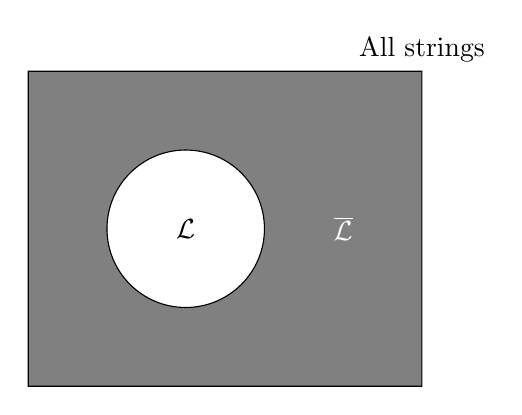
\begin{tikzpicture}[fill=gray]
    \scope
      \clip (-2, -2) rectangle (3, 2)
            (0, 0) circle (1);
      \fill (-2, -2) rectangle (3, 2);
    \endscope
    \scope
      \clip (-2, -2) rectangle (3, 2)
            (0, 0) circle (1);
      \fill (0, 0) circle (1);
    \endscope
    \draw (0, 0) circle (1) (0, 0) node [text = black] {$\mathcal L$}
          (2, 0) node [text = white] {$\overline{\mathcal L}$}
          (-2, -2) rectangle (3, 2) node [text = black, above] {All strings};
  \end{tikzpicture}
\end{center}

\begin{defn}
  The {\boldmath \bfseries complement}  of the language $\mathcal L$ is 
  \[
    \overline{\mathcal L} = \left \{ w : w \not \in \mathcal L \right \}.
  \]
\end{defn}

\begin{thm}
  If $\mathcal L$ is regular then $\overline{\mathcal L}$ is regular.
  In other words, regular languages are closed under complement.
\end{thm}

\begin{prf}
  Swap the accept and reject states of the DFA for $\mathcal L$ to get a DFA for $\overline{\mathcal L}$.

  Formally, if DFA $(Q, \Sigma, \delta, q_0, F)$ recognizes $\mathcal L$ then DFA $(Q, \Sigma, \delta, q_0, Q \setminus F)$ recognizes $\overline{\mathcal L}$.
\end{prf}

\begin{eg}
  $\mathcal L = \left \{ w : w \neq \verb~0~, \verb~1~ \right \}$.
  
  Note that $\overline{\mathcal L} = \left \{ w : w = \verb~0~ \lor w = \verb~1~ \right \}$.
  The DFA for $\overline{\mathcal L}$ is given by: 

  \begin{center}
    \begin{tikzpicture}[> = stealth, node distance = 3em]
      \node[initial, initial text=, state, minimum size = 2em] (0) {};
      \node[right = of 0, accepting, state, minimum size = 2em] (1) {};
      \node[right = of 1, state, minimum size = 2em] (2) {};
      \draw[->]
      (0) edge[above] node{\verb~0~,\verb~1~} (1)
      (1) edge[above] node{\verb~0~,\verb~1~} (2)
      (2) edge[loop right] node{\verb~0~,\verb~1~} (2)
      ;
    \end{tikzpicture}
  \end{center}
  
  Then the DFA for $\mathcal L$ is given by 

  \begin{center}
    \begin{tikzpicture}[> = stealth, node distance = 3em]
      \node[accepting, initial, initial text=, state, minimum size = 2em] (0) {};
      \node[right = of 0, state, minimum size = 2em] (1) {};
      \node[accepting, right = of 1, state, minimum size = 2em] (2) {};
      \draw[->]
      (0) edge[above] node{\verb~0~,\verb~1~} (1)
      (1) edge[above] node{\verb~0~,\verb~1~} (2)
      (2) edge[loop right] node{\verb~0~,\verb~1~} (2)
      ;
    \end{tikzpicture}
  \end{center}
\end{eg}

\begin{eg}
  $\mathcal L = \left \{ w : \text{$w$ does not contain \verb~0101~} \right \}$.
  
  Note that $\overline{\mathcal L} = \left \{ w : \text{$w$ contains \verb~0101~} \right \}$.
  The DFA for $\overline{\mathcal L}$ is given by: 

  \begin{center}
    \begin{tikzpicture}[> = stealth, node distance = 3em]
      \node[initial, initial text=, state, minimum size = 2em] (0) {};
      \node[right = of 0, state, minimum size = 2em] (1) {};
      \node[right = of 1, state, minimum size = 2em] (2) {};
      \node[right = of 2, state, minimum size = 2em] (3) {};
      \node[accepting, right = of 3, state, minimum size = 2em] (4) {};
      \draw[->]
      (0) edge[loop below] node{\verb~1~} (0)
      (0) edge[above] node{\verb~0~} (1)
      (1) edge[loop below] node{\verb~0~} (1)
      (1) edge[above] node{\verb~1~} (2)
      (2) edge[above] node{\verb~0~} (3)
      (2) edge[bend right, above] node{\verb~1~} (0)
      (3) edge[above] node{\verb~1~} (4)
      (3) edge[bend right, above] node{\verb~0~} (1)
      (4) edge[loop below] node{\verb~0~,\verb~1~} (4)
      ;
    \end{tikzpicture}
  \end{center}
  
  Then the DFA for $\mathcal L$ is given by 

  \begin{center}
    \begin{tikzpicture}[> = stealth, node distance = 3em]
      \node[accepting, initial, initial text=, state, minimum size = 2em] (0) {};
      \node[accepting, right = of 0, state, minimum size = 2em] (1) {};
      \node[accepting, right = of 1, state, minimum size = 2em] (2) {};
      \node[accepting, right = of 2, state, minimum size = 2em] (3) {};
      \node[right = of 3, state, minimum size = 2em] (4) {};
      \draw[->]
      (0) edge[loop below] node{\verb~1~} (0)
      (0) edge[above] node{\verb~0~} (1)
      (1) edge[loop below] node{\verb~0~} (1)
      (1) edge[above] node{\verb~1~} (2)
      (2) edge[above] node{\verb~0~} (3)
      (2) edge[bend right, above] node{\verb~1~} (0)
      (3) edge[above] node{\verb~1~} (4)
      (3) edge[bend right, above] node{\verb~0~} (1)
      (4) edge[loop below] node{\verb~0~,\verb~1~} (4)
      ;
    \end{tikzpicture}
  \end{center}
\end{eg}

\subsection{Union and intersection}

\begin{minipage}{0.5 \textwidth}
  \begin{center}
    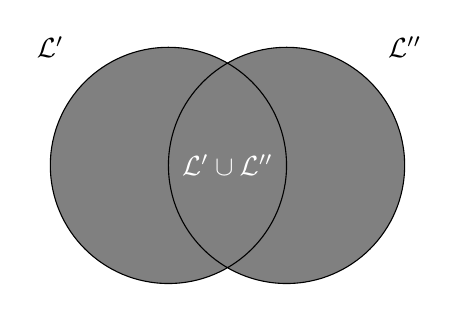
\begin{tikzpicture}[fill=gray]
      \fill (0, 0) circle (1.5);
      \fill (1.5, 0) circle (1.5);
      \draw (0, 0) circle (1.5) (-1.5, 1.5) node[text = black]{$\mathcal L'$}
            (1.5, 0) circle (1.5) (3, 1.5) node[text = black] {$\mathcal L''$}
            (0.75, 0) node[text = white]{$\mathcal L' \cup \mathcal L''$};
    \end{tikzpicture}
  \end{center}
\end{minipage}%
\begin{minipage}{0.5 \textwidth}
  \begin{center}
    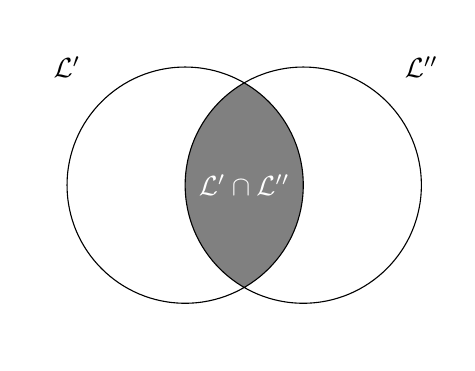
\begin{tikzpicture}[fill=gray]
      \scope
        \clip (-2, -2) rectangle (3, 2)
              (1.5, 0) circle (1.5)
              (0, 0) circle (1.5);
        \fill (0, 0) circle (1.5);
      \endscope
      \draw (0, 0) circle (1.5) (-1.5, 1.5) node[text = black]{$\mathcal L'$}
            (1.5, 0) circle (1.5) (3, 1.5) node[text = black] {$\mathcal L''$}
            (0.75, 0) node[text = white]{$\mathcal L' \cap \mathcal L''$};
    \end{tikzpicture}
  \end{center}
\end{minipage}

\begin{defn}
  The {\boldmath \bfseries union} of languages $\mathcal L'$ and $\mathcal L''$ is 
  \[
    \mathcal L' \cup \mathcal L'' = \left \{ w : w \in \mathcal L' \lor w \in \mathcal L'' \right \}.
  \]
\end{defn}

\begin{defn}
  The {\boldmath \bfseries intersection} of languages $\mathcal L'$ and $\mathcal L''$ is 
  \[
    \mathcal L' \cap \mathcal L'' = \left \{ w : w \in \mathcal L' \land w \in \mathcal L'' \right \}.
  \]
\end{defn}

\begin{thm}
  If $\mathcal L'$, $\mathcal L''$ are regular, then so are 
  \begin{oldenumerate}[topsep = 0ex, label = {(\alph*)}]
    \item $\mathcal L' \cup \mathcal L''$ and 

    \item $\mathcal L' \cap \mathcal L''$.
  \end{oldenumerate}
  
  In other words, regular lanaguages are closed under union and intersection.
\end{thm}

\begin{prf}
  \begin{oldenumerate}[topsep = 0ex, label = {(\alph*)}]
    \item Connect an initial state to the initial states for the NFAs for $\mathcal L'$ and $\mathcal L''$ via $\varepsilon$.
      
    \item If $\mathcal L'$ and $\mathcal L''$ are regular then $\overline{\mathcal L'}$ and $\overline{\mathcal L''}$ are regular.
    Then $\overline{\mathcal L'} \cup \overline{\mathcal L''}$ is regular.
    Then, by De Morgan's law, $\mathcal L' \cap \mathcal L'' = \overline{\overline{\mathcal L'} \cup \overline{\mathcal L''}}$ is regular.
  \end{oldenumerate}
\end{prf}

\begin{prf}
  {\boldmath \bfseries Idea: }\footnote{Here ``E'' stands for ``EVEN'', ``O'' stands for ``ODD'', ``H'' stands for ``HAPPY'', ``W'' stands for ``WORRIED'', and ``S'' stands for ``SAD''.}
  
  \begin{minipage}{0.48 \textwidth}
    \begin{center}
      $\mathcal L' = \left \{ w : \text{$w$ has an even number of \verb~0~s} \right \}$.
    \end{center}
  \end{minipage}%
  \hfill%
  \begin{minipage}{0.48 \textwidth}
    \begin{center}
      $\mathcal L'' = \left \{ w : \text{every \verb~0~ is immediately followed by a \verb~1~} \right \}$.
    \end{center}
  \end{minipage}
  \vspace{0.5 \baselineskip}

  \begin{minipage}{0.45 \textwidth}
    \begin{center}
      \begin{tikzpicture}[> = stealth, node distance = 3em]
        \node[accepting, initial, initial text=, state, minimum size = 2em] (e) {E};
        \node[below = of e, state, minimum size = 2em] (o) {O};
        \draw[->]
        (e) edge[bend right, left] node{\verb~0~} (o)
        (e) edge[loop right] node{\verb~1~} (e)
        (o) edge[bend right, right] node{\verb~0~} (e)
        (o) edge[loop right] node{\verb~1~} (o)
        ;
      \end{tikzpicture}
    \end{center}
  \end{minipage}%
  \hfill%
  \begin{minipage}{0.45 \textwidth}
    \begin{center}
      \begin{tikzpicture}[> = stealth, node distance = 3em]
        \node[accepting, initial, initial text=, state, minimum size = 2em] (h) {H};
        \node[right = of h, state, minimum size = 2em] (w) {W};
        \node[right = of w, state, minimum size = 2em] (s) {S};
        \draw[->]
        (h) edge[loop above] node{\verb~1~} (h)
        (h) edge[bend right, below] node{\verb~0~} (w)
        (w) edge[bend right, above] node{\verb~1~} (h)
        (w) edge[above] node{\verb~0~} (s)
        (s) edge[loop above] node{\verb~0~,\verb~1~} (s)
        ;
      \end{tikzpicture}
    \end{center}
  \end{minipage}
  \vspace{0.5 \baselineskip}
  
  Consider the construction: 

  \begin{center}
    \begin{tikzpicture}[> = stealth, node distance = 3em]
      \node[initial below, initial text=, state, minimum size = 2em] (eh) {E, H};
      \node[right = of eh, state, minimum size = 2em] (ew) {E, W};
      \node[right = of ew, state, minimum size = 2em] (es) {E, S};
      \node[below = of eh, state, minimum size = 2em] (oh) {O, H};
      \node[right = of oh, , state, minimum size = 2em] (ow) {O, W};
      \node[right = of ow, state, minimum size = 2em] (os) {O, S};
      \draw[->]
      (eh) edge[loop left] node{\verb~1~} (eh)
      (eh) edge[] node[above left = 0 and 0.3, sloped]{\verb~0~} (ow)
      (ew) edge[above] node{\verb~1~} (eh)
      (ew) edge[] node[above left = 0 and 0.3, sloped]{\verb~0~} (os)
      (es) edge[loop right] node{\verb~1~} (es)
      (es) edge[bend right, left] node{\verb~0~} (os)
      (oh) edge[loop left] node{\verb~1~} (oh)
      (oh) edge[] node[above left = 0 and 0.3, sloped]{\verb~0~} (ew)
      (ow) edge[above] node{\verb~1~} (oh)
      (ow) edge[] node[above left = 0 and 0.3,  sloped]{\verb~0~} (es)
      (os) edge[loop right] node{\verb~0~} (os)
      (os) edge[bend right, right] node{\verb~0~} (es)
      ;
    \end{tikzpicture}
  \end{center}

  Note that we can create DFAs for either union or intersection by assigning appropriate accept states: 

  \begin{minipage}{0.45 \textwidth}
    \begin{center}
      $\mathcal L = \mathcal L' \cup \mathcal L''.$
    \end{center}
  \end{minipage}%
  \hfill%
  \begin{minipage}{0.45 \textwidth}
    \begin{center}
      $\mathcal L = \mathcal L' \cap \mathcal L''.$
    \end{center}
  \end{minipage}
  \vspace{0.5 \baselineskip}

  \begin{minipage}{0.45 \textwidth}
    \begin{center}
      \scalebox{0.8}{
        \begin{tikzpicture}[> = stealth, node distance = 3em]
          \node[accepting, initial below, initial text=, state, minimum size = 2em] (eh) {E, H};
          \node[accepting, right = of eh, state, minimum size = 2em] (ew) {E, W};
          \node[accepting, right = of ew, state, minimum size = 2em] (es) {E, S};
          \node[accepting, below = of eh, state, minimum size = 2em] (oh) {O, H};
          \node[right = of oh, , state, minimum size = 2em] (ow) {O, W};
          \node[right = of ow, state, minimum size = 2em] (os) {O, S};
          \draw[->]
          (eh) edge[loop left] node{\verb~1~} (eh)
          (eh) edge[] node[above left = 0 and 0.3, sloped]{\verb~0~} (ow)
          (ew) edge[above] node{\verb~1~} (eh)
          (ew) edge[] node[above left = 0 and 0.3, sloped]{\verb~0~} (os)
          (es) edge[loop right] node{\verb~1~} (es)
          (es) edge[bend right, left] node{\verb~0~} (os)
          (oh) edge[loop left] node{\verb~1~} (oh)
          (oh) edge[] node[above left = 0 and 0.3, sloped]{\verb~0~} (ew)
          (ow) edge[above] node{\verb~1~} (oh)
          (ow) edge[] node[above left = 0 and 0.3,  sloped]{\verb~0~} (es)
          (os) edge[loop right] node{\verb~0~} (os)
          (os) edge[bend right, right] node{\verb~0~} (es)
          ;
        \end{tikzpicture}
      }
    \end{center}
  \end{minipage}%
  \hfill%
  \begin{minipage}{0.45 \textwidth}
    \begin{center}
      \scalebox{0.8}{
        \begin{tikzpicture}[> = stealth, node distance = 3em]
          \node[accepting, initial below, initial text=, state, minimum size = 2em] (eh) {E, H};
          \node[right = of eh, state, minimum size = 2em] (ew) {E, W};
          \node[right = of ew, state, minimum size = 2em] (es) {E, S};
          \node[below = of eh, state, minimum size = 2em] (oh) {O, H};
          \node[right = of oh, , state, minimum size = 2em] (ow) {O, W};
          \node[right = of ow, state, minimum size = 2em] (os) {O, S};
          \draw[->]
          (eh) edge[loop left] node{\verb~1~} (eh)
          (eh) edge[] node[above left = 0 and 0.3, sloped]{\verb~0~} (ow)
          (ew) edge[above] node{\verb~1~} (eh)
          (ew) edge[] node[above left = 0 and 0.3, sloped]{\verb~0~} (os)
          (es) edge[loop right] node{\verb~1~} (es)
          (es) edge[bend right, left] node{\verb~0~} (os)
          (oh) edge[loop left] node{\verb~1~} (oh)
          (oh) edge[] node[above left = 0 and 0.3, sloped]{\verb~0~} (ew)
          (ow) edge[above] node{\verb~1~} (oh)
          (ow) edge[] node[above left = 0 and 0.3,  sloped]{\verb~0~} (es)
          (os) edge[loop right] node{\verb~0~} (os)
          (os) edge[bend right, right] node{\verb~0~} (es)
          ;
        \end{tikzpicture}
      }
    \end{center}
  \end{minipage}
  \vspace{0.5 \baselineskip}
  
  Note that this construction is better than that in the first proof since the number of nodes in this construction is $\mathcal O(n^2)$ while that in the first proof is $\mathcal O(4^n)$.
  
  Formally, write the DFA for $\mathcal L'$ as $(Q', \Sigma, \delta', q_0', F')$ and that for $\mathcal L''$ as $(Q'', \Sigma, \delta'', q_0'', F'')$.
  
  Then the DFA for $\mathcal L' \cup \mathcal L''$ is given by $(Q' \times Q'', \Sigma, \delta, (q_0', q_0''), (F' \times Q'') \cup (Q' \times F''))$ where $\delta((q', q''), \sigma) := (\delta'(q', \sigma), \delta''(q'', \delta))$ for all $q' \in Q'$, $q'' \in Q''$, and $\sigma \in \Sigma$.

  Similarly, the DFA for $\mathcal L' \cap \mathcal L''$ is given by $(Q' \times Q'', \Sigma, \delta, (q_0', q_0''), F' \times F'')$ where \\ $\delta((q', q''), \sigma) := (\delta'(q', \sigma), \delta''(q'', \delta))$ for all $q' \in Q'$, $q'' \in Q''$, and $\sigma \in \Sigma$.
\end{prf}

\begin{cor}
  If $\mathcal L_1, \mathcal L_2, \dots, \mathcal L_n$ are regular, so are 
  \begin{itemize}
    \item $\mathcal L_1 \cup \mathcal L_2 \cup \cdots \cup \mathcal L_n$ and 

    \item $\mathcal L_1 \cap \mathcal L_2 \cap \cdots \cap \mathcal L_n$.
  \end{itemize}
\end{cor}

\begin{prf}
  Induction.
\end{prf}

\begin{cor}
  Every finite language is regular.
\end{cor}

\begin{prf}
  Let $\mathcal L$ be finite.
  Then we can write 
  \[
    \mathcal L = \bigcup_{w \in \mathcal L} \left \{ w \right \}, 
  \]
  that is, as a union of singleton languages.

  Note that an NFA can be easily found for any singleton language, that is, singleton languages are regular.
  Then $\mathcal L$ is regular by Corollary~\ref{cor:4.2.4}.
\end{prf}

\end{document}